\chapter{Developing Glazes}
Most potters do not know much about glaze chemistry and are usually afraid to 
develop their own glazes. It is true that glaze chemistry is difficult to 
understand without a background in chemistry. Still, a simple knowledge of 
fluxes, stabilizers and glass formers and how they combine to make glaze is 
useful. It will give even the nontechnical potter an idea of how to approach 
glaze problems and develop new colors and textures. The reader with more 
technical background can make use of the Seger formula for a more sophisticated 
approach to glazes.

Remember that glaze chemistry is something new in the history of ceramics. 
Before it existed, potters found out how to make glazes by trial and error, 
without modern methods of analysis or even accurate methods of weighing.

It is also true that once glaze recipes were developed they were closely 
guarded secrets. A special glaze that no one else could duplicate gave an 
advantage over the competition. The modern systematic, scientific approach to 
glaze development has largely made ``secret'' glazes obsolete because the 
action of the various glaze ingredients is now well known.

On the other hand, glaze making is very much like cooking. The same recipe may 
produce very different results when prepared by two different cooks! Standard 
glaze recipes as published in books often do not work because of differences in 
raw materials, firing technique etc. Just as a good cook should know how to 
substitute materials, a good glaze maker can develop an intuitive knowledge of 
glazes. Like most things, this only comes from hard-won experience.

Potters should not be afraid to experiment with glaze development, although 
most of them simply do not have the time to take away from production. The 
following chapters describe standard approaches to glaze development and will 
be useful to those who want to experiment with glazes.
%------------------------------------------------------------------------------
\section{Modifying Existing Glazes}
The easiest approach to working with glazes is to start by modifying existing 
glazes. These may be new recipes from books, or recipes that you are already 
using. Although you can take a trial-and-error approach, this takes a lot of 
time and money, and results are largely a matter of luck. It is best to use 
some of the systematic methods presented below and knowing even a little about 
the nature of the various glaze materials will help you reach your goal more 
efficiently.

There are three approaches to modifying glazes:
%------------------------------------------------------------------------------
\begin{itemize}
\item You have a goal for a particular surface, color, texture etc.
\item You have a glaze problem that needs to be corrected.
\item You have no special goal but just want to see what happens when you 
change the recipe.
\end{itemize}
%------------------------------------------------------------------------------
\section{Basic Equipment}
The minimum equipment required for glaze testing is:
%------------------------------------------------------------------------------
\begin{itemize}
\item Accurate balance, either a triple beam balance or a goldsmith's balance 
with weight. Spring-type scales are not accurate enough for weighing glazes.
\item A mortar and pestle for grinding materials. These should be porcelain, so 
that they do not contaminate tests.
\item A 100-mesh sieve. This can be bought ready-made, or you can make your own 
using brass or stainless steel screen.
\item Firing can be done in your regular glaze firing.
\end{itemize}
%------------------------------------------------------------------------------
\section{Testing Methods}
\subsection{Test Pieces}
The type of test piece you use is largely a matter of personal preference. In 
order to show glaze behavior under various circumstances, it should have:
%------------------------------------------------------------------------------
\begin{itemize}
\item A horizontal and vertical surface.
\item A textured area.
\item A hole to tie it. This helps to keep similar tests together for future 
reference.
\item An area for labeling. It is best to write the full recipe of the test on 
each test tile (with a brush and iron oxide and water, or chrome oxide or 
engobe etc.) since code numbers often get confused and notebooks get lost.
\end{itemize}
%------------------------------------------------------------------------------
The first step in understanding your materials is to fire all available 
materials in small bowls at your standard glaze firing temperature.

A small quantity of each material (ground and sieved through 100 mesh) is 
placed dry in the bowl. This will show you which ones melt alone, and which 
ones remain as powder. Most of the materials will not melt but may change in 
color or may react with the clay. Only the strong fluxes will melt by 
themselves -other materials that do not melt may be fluxes, but only in 
combination with other materials.
%------------------------------------------------------------------------------
\subsection{Line Blending}
Line blending is a systematic way of finding out the reactions of two different 
materials (or mixtures of materials).

The easiest way is to prepare the two materials by grinding, sieving and mixing 
them with water in two separate containers. To make the line blend, the 
materials are mixed by volume (using a small spoon) and applied on a test tile, 
starting with one material alone and adding the other material in equal steps. 
Since the tests are measured by volume it is important that the same amount of 
water is added to the two line blend materials.

Glaze half of the test tile twice to show variation in glaze thickness.

An example of a line blend in 10 steps, which gives the full range of 
combinations of 2 materials, is shown in table~\ref{tab:lineblend10}.

The most common use of the line blend is to find out the effect of one material 
in a standard glaze recipe. If material A is the standard glaze recipe, 
material B could be the standard glaze + a coloring oxide addition of 5-10%.

Usually, 5 steps will be enough for the first test. In 
table~\ref{tab:lineblend5ox}, material A is the basic glaze, material B is the 
basic glaze + 10\% copper oxide.
%------------------------------------------------------------------------------
\begin{center}
  \begin{table}\centering
  \renewcommand{\arraystretch}{1.5}    
  \begin{tabular}{|c||c|c|c|c|c|c|c|c|c|c|c|}\hline
      \textbf{Material}
      &\multicolumn{11}{c}{\textbf{Parts by volume}}\vline\\\hline\hline
      Material A&0&1&2&3&4&5&6&7&8&9&10\\\hline
      Material B&10&9&8&7&6&5&4&3&2&1&0\\\hline
    \end{tabular}
  \caption{A line blend of 10 steps.}
\label{tab:lineblend10}
  \end{table}
\end{center}
%------------------------------------------------------------------------------
\begin{center}
  \renewcommand{\arraystretch}{1.5}
  \begin{table}\centering
    \begin{tabular}{|c||c|c|c|c|c|c|}\hline
      \textbf{Material}&\multicolumn{6}{c}{\textbf{Parts by 
      volume}}\vline\\\hline\hline
      \textbf{Test}
    &\textbf{A}&\textbf{B}&\textbf{C}&\textbf{D}&\textbf{E}&\textbf{F}\\\hline\hline
      Glaze A&0&2&4&6&8&10\\\hline
      Glaze A + 10\% \ce{CuO}&10&8&6&4&2&0\\\hline
      \ce{CuO} in test&10\%&8\%&6\%&4\%&2\%&0\%\\\hline
     \end{tabular}
    \caption{A line blend of 5 steps, mixing glazes and an oxide.}
    \label{tab:lineblend5ox}
  \end{table}
\end{center}
%------------------------------------------------------------------------------
\subsubsection{Mixing procedure}
\begin{enumerate}
\item First prepare a line blend mixing card like the one above.
\item Prepare the two mixtures as usual and add the same amount of water to 
each.
\item Place the two materials in bowls in front of you, glaze A to your left 
and glaze B to your right.
\item In the middle place an empty bowl into which you pour the spoonfuls from 
the two other bowls according to the number for each test on your line blend 
card. Keep track of the spoon counting by marking the line blend card.
\item Stir the test mixture well.
\item Mark a test tile with the mixture's test number (date + serial number).
\item Glaze the test tile.
\item Discard the remaining glaze and continue with the other line blend 
mixtures.
\end{enumerate}

\subsubsection{Calculation example}
In the case above it was easy to calculate the copper oxide addition in each of 
the tests. When more complex mixtures are used in a line blend the calculation 
becomes more complicated. 

Table~\ref{tab:lineblend5} shows an example of mixing two glazes of the 
following compositions:
\begin{itemize}
\item Glaze A:
\begin{itemize}
\item Frit X: 70
\item Feldspar: 15
\item Quartz: 5
\item Kaolin: 10
\end{itemize}
\item Glaze B
\begin{itemize}
  \item Frit Y: 80
  \item Zircon: 10
  \item Kaolin: 10
\end{itemize}
\end{itemize}
%------------------------------------------------------------------------------
\begin{center}
  \renewcommand{\arraystretch}{1.5}
  \begin{table}\centering
    \begin{tabular}{|c||c|c|c|c|c|c|}\hline
      &\multicolumn{6}{c}{\textbf{Parts by volume}}\vline\\\hline\hline
      \textbf{Test Number}
      &\textbf{A}&\textbf{B}&\textbf{C}&\textbf{D}&\textbf{E}&\textbf{F}\\\hline\hline
      Glaze A&0&2&4&6&8&10\\\hline
      Glaze B&10&8&6&4&2&0\\\hline
    \end{tabular}
    \caption{A line blend of 5 steps.}
    \label{tab:lineblend5}
  \end{table}
\end{center}
%------------------------------------------------------------------------------
After firing, Test D turned out to be the most interesting. We now want 
to test a larger amount of this and the recipe is calculated as shown in 
table~\ref{tab:lineblendtestd}.

The sums of each material were then divided by 5 and the final recipe is shown 
in table~\ref{tab:lineblendglazed}.

The recipe is based on a line blend test measured by spoonfuls. That is not 
very accurate so, before going any further, the test result should be retested 
by weighing the dry materials.
%------------------------------------------------------------------------------
\begin{landscape}
  \begin{center}
  \renewcommand{\arraystretch}{1.5}
  \begin{table}\centering
    \begin{tabular}{|c||c|c|c|c|c|c|c|}\hline
      &\textbf{Parts}&\textbf{Frit X}&\textbf{Frit 
      Y}&\textbf{Feldspar}&\textbf{Quartz}&\textbf{Zircon}&\textbf{Kaolin}\\\hline\hline
      Glaze A&3&210&0&45&15&0&30\\\hline
      Glaze B&2&0&160&0&0&20&20\\\hline
      Total A+B&5&210&160&45&15&20&50\\\hline\hline
      New Glaze D&0.2&42&32&9&3&4&10\\\hline
    \end{tabular}
    \caption{The composition of Test D. Materials in Glaze A were multiplied by 
    3, and Glaze B by 2.}
    \label{tab:lineblendtestd}
  \end{table}
\end{center}
\end{landscape}
%------------------------------------------------------------------------------
\begin{center}
  \renewcommand{\arraystretch}{1.5}
  \begin{table}\centering
    \begin{tabular}{|c|c|}\hline
      \textbf{Ingredient}&\textbf{Percent}\\\hline\hline
      Frit X&42\%\\\hline
      Frit Y&32\%\\\hline
      Feldspar&9\%\\\hline
      Quartz&3\%\\\hline
      Zircon&4\%\\\hline
      Kaolin&10\%\\\hline
    \end{tabular}
    \caption{Glaze D, final recipe.}
    \label{tab:lineblendglazed}
  \end{table}
\end{center}
%------------------------------------------------------------------------------
\subsection{Triaxial Blending}
Triaxial blending is a method of testing varying amounts of three different 
materials or colors.
%-------------------------------------------------------------------------------
\begin{figure}[htbp!]
  \centering
  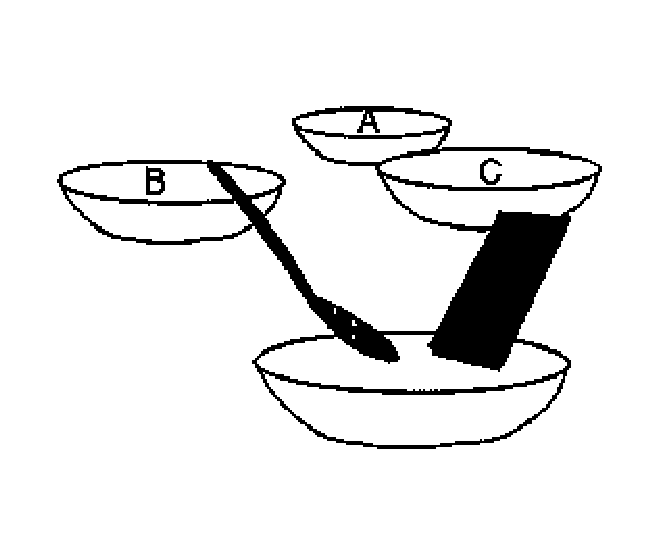
\includegraphics[width=0.7\linewidth]{img/triaxialbowls.eps}
  \caption{Arrangement of bowls for triaxial mixing.}
  \label{fig:triaxialbowls}
\end{figure}
%-------------------------------------------------------------------------------
\begin{figure}[htbp!]
  \centering
  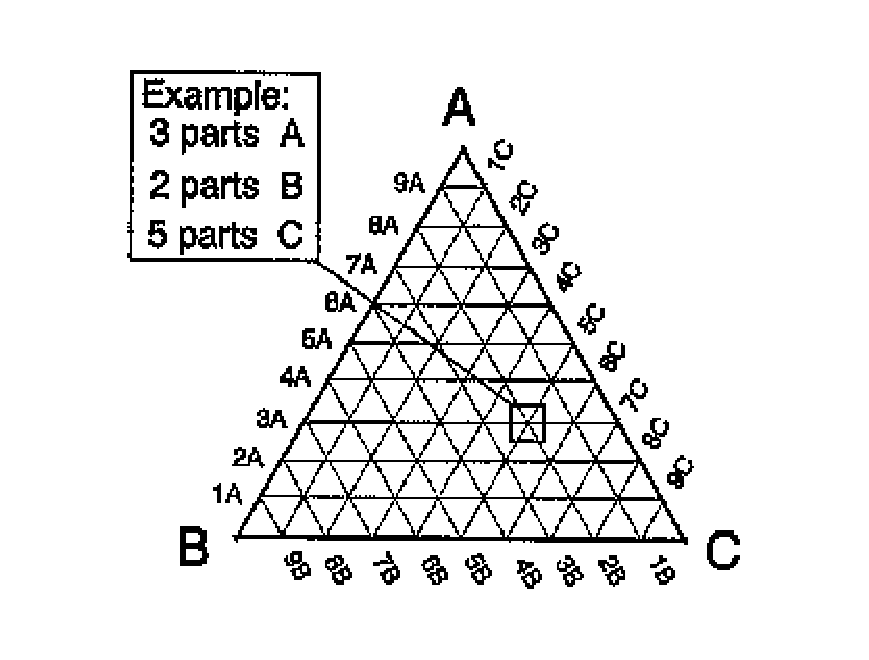
\includegraphics[width=0.7\linewidth]{img/triaxial10.eps}
  \caption{A triaxial blending chart system with 10 steps. Composition of a 
    test at an intersection is found by following the lines to the periphery of 
    the triangle.}
  \label{fig:triaxial10}
\end{figure}
%-------------------------------------------------------------------------------
\begin{figure}[htbp!]
  \centering
  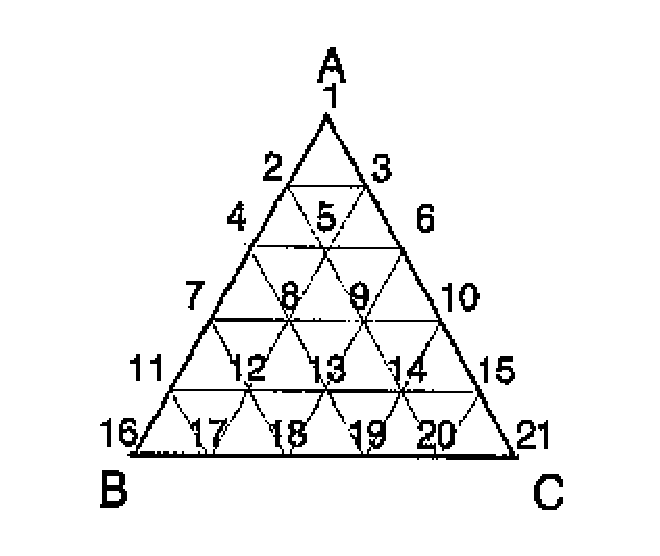
\includegraphics[width=0.7\linewidth]{img/triaxial5.eps}
  \caption{Triaxial system with 5 steps. The number at each point refers to the 
    test number on the triaxial blending card.}
  \label{fig:triaxial5}
\end{figure}
%-------------------------------------------------------------------------------
Each corner of the triangle represents 100\% of the material. Each side of the 
triangle is the line blend of the materials at its ends, and the intersections 
inside the triangle represent combinations of all three materials. So the 
result is three line blends, plus all the combinations. 

Figure~\ref{fig:triaxial10} is an example of a biaxial system with 66 tests.

The system is better explained by an example. You may have a basic opaque glaze 
and you want to see how it responds to 3 different coloring oxides: cobalt 
oxide, copper oxide and iron oxide. In this case we use a simple biaxial blend 
with only 21 tests as shown in figure~\ref{fig:triaxial5}.

The procedure is:
%-------------------------------------------------------------------------------
\begin{itemize}
\item Prepare a biaxial blending card as shown.
\item Prepare 3 mixtures of basic glaze with oxide additions:
%-------------------------------------------------------------------------------
\begin{itemize}
\item A glaze + 5\% cobalt oxide
\item B glaze + 10\% iron oxide
\item C glaze + 10\% copper oxide
\end{itemize}
%-------------------------------------------------------------------------------
\item Add same amount of water, screen 100 mesh.
\item Place 3 bowls with the mixtures in front of you: B on the left, C on the 
right, A in the center. Right in front of you place an empty bowl. See 
figure~\ref{fig:triaxialbowls}
\item Have all test tiles numbered and arranged in sequence near by.
\item Collect teaspoonfuls of each mixture; A, B, C according to the numbers on 
the biaxial card. Mark each time you have finished collecting from each bowl.
\item The mixture is collected in the empty bowl.
\item Stir the mixture, pick the test tile with the right biaxial blend number.
\item Glaze the test tile.
\end{itemize}
%-------------------------------------------------------------------------------
Getting the right number of spoonfuls into the collection bowl for each test 
takes a lot of concentration. A mixing card as shown in 
table~\ref{tab:mixingcard} helps you to keep track of your progress with the 
spoon counting.
%-------------------------------------------------------------------------------
\begin{landscape}
\begin{center}
  \begin{table}\centering
  \renewcommand{\arraystretch}{1.5}
  \begin{tabular}{|c||c|c|c|c|c|c|c|c|c|c|c|c|c|c|c|c|c|c|c|c|c|}\hline
    &\multicolumn{21}{c}{\textbf{Triaxial Blending Card}}\vline\\\hline\hline
    \textbf{Test Number}
    &\textbf{1}&\textbf{2}&\textbf{3}&\textbf{4}&\textbf{5}&\textbf{6}
    &\textbf{7}&\textbf{8}&\textbf{9}&\textbf{10}&\textbf{11}&\textbf{12}&\textbf{13}
    &\textbf{14}&\textbf{15}&\textbf{16}&\textbf{17}&\textbf{18}&\textbf{19}
    &\textbf{20}&\textbf{21}\\\hline\hline
    Material&\multicolumn{21}{c}{Number of Spoonfulls}\vline\\\hline\hline
    Mixture A&5&4&4&3&3&3&2&2&2&2&1&1&1&1&1&0&0&0&0&0&0\\\hline
    Mixture B&0&1&0&2&1&0&3&2&1&0&4&3&2&1&0&5&4&3&2&1&0\\\hline
    Mixture C&0&0&1&0&1&2&0&1&2&3&0&1&2&3&4&0&1&2&3&4&5\\\hline
  \end{tabular}
  \caption{A blending card for a triaxial blend.}
  \label{tab:mixingcard}
\end{table}
  \end{center}
\end{landscape}
%-------------------------------------------------------------------------------
If you want to know the recipe of one of the tests, say number 14, you 
calculate this in the same way as for line blends. See 
table~\ref{tab:lineblend14}. Once you get used to working with biaxial blends, 
you will be able to read the percentage directly from the triangular chart.

This biaxial blend was based on only 21 variations. Out of these only 6 were 
blendings of all three mixtures; the rest were simply line blends involving 
only two mixtures. A larger biaxial blend system would produce more intermixing 
of all three materials, but also a lot of extra work. However, you could use a 
system with 10 steps on each side as shown in 
figure~\ref{fig:glazetestrecordform}, but leaving out the line blends A--B, 
A--C and B--C, and only blend the 36 
tests in the center of the triangle.
%-------------------------------------------------------------------------------
\begin{figure}[htbp!]
  \centering
  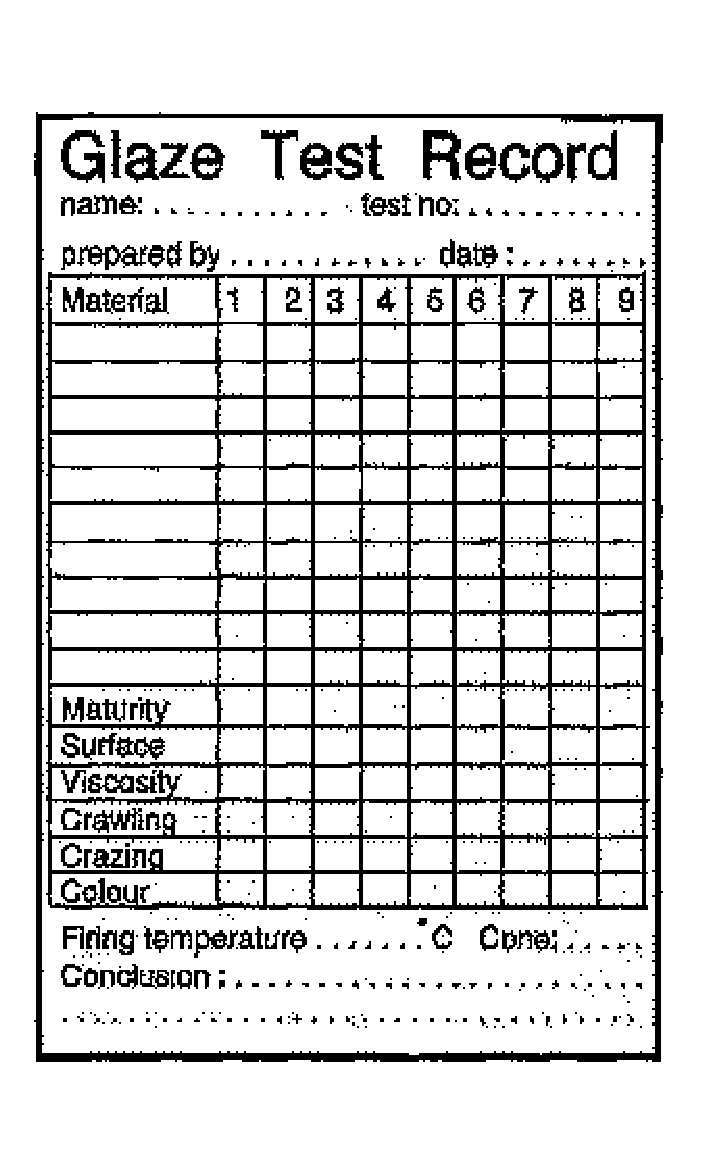
\includegraphics[width=0.45\linewidth]{img/glazetestrecordform.eps}
  \caption{Example of a glaze test record form.}
  \label{fig:glazetestrecordform}
\end{figure}
%-------------------------------------------------------------------------------
\begin{landscape}
  \begin{center}
\begin{table}\centering
    \renewcommand{\arraystretch}{1.5}
\begin{tabular}{|c||c|c|c|c|c|c|}\hline
&&\textbf{Parts}&\textbf{Glaze}&\textbf{Cobalt Oxide}&\textbf{Iron 
Oxide}&\textbf{Copper Oxide}\\\hline\hline
\textbf{Mixture A}&1&100&5&0&0&0\\\hline
\textbf{Mixture B}&1&100&0&0&10&0\\\hline
\textbf{Mixture C}&3&300&0&0&0&30\\\hline
\textbf{Total}&-&5&500&5&10&30\\\hline
\textbf{Recipe D}&Total/5&100\%&+1\%&0&+2\%&+6\%\\\hline
\end{tabular}
  \caption{A line blend of test number 14.}
\label{tab:lineblend14}
\end{table}
\end{center}
\end{landscape}
%-------------------------------------------------------------------------------
\subsection{Keeping Records}
The key to experimenting with glazes is keeping accurate records and labeling 
them in such a way that the actual tests can be compared with your notebook.

As mentioned above, it is best to write the entire recipe on the test tile 
itself, along with the date of testing. This is possible with a simple test 
like adding coloring oxides to your basic glaze. For more complicated tests and 
line blend or biaxial blend tests, you will have to rely on the test number on 
the tile. Mark the date, the number and, if you do more than one test a day, 
add a serial number. In your notebook, the date and recipe are also written.

Make it a habit to take notes of the fired results immediately after unloading 
the kiln. Write down firing conditions, location of test tile in the kiln, and 
your impression of the glaze. Is it well melted, running, pinholes or tendency 
to crawl? Use a whole sheet of paper for each test or test series. Finally 
write down your conclusion like ``make 1 kg test batch'', ``test again with 5\% 
increase of clay''.

Testing is costly and the records help you to avoid unnecessary tests. When 
planning your next test, first take a look at your earlier results and compare 
them with your notes. When deciding which materials to add or which to decrease 
you may check with the oxide list (see section~\ref{sec:glazeoxides}). As long 
as you work with one particular problem or line of research keep the test tiles 
close by for easy reference. Once you have finished the research you can store 
all the tests together by hanging them on a string in chronological order.
%-------------------------------------------------------------------------------
\section{Developing a Base Glaze}
The first step in developing a new glaze is to develop a base glaze, which is 
simply the combination of materials that melts at the desired temperature 
(without addition of colorants). Here, we describe an approach to making base 
glazes without knowing anything about the chemical composition of the materials.

Since all glazes require flux, stabilizer and glass former, these three 
materials are the starting point. There are a large number of fluxes available 
(divided into primary and secondary' fluxes), but the stabilizer is usually 
china clay (kaolin) and the glass former is usually quartz (silica). The main 
differences are between low temperature and high temperature glazes. Below only 
the main materials (not chemicals) are mentioned. This list is a rough guide 
only.

\subsection{Low Temperature Glazes (900--1100\degree C)}
Low temperature glazes require more flux and stronger flux than high 
temperature ones.

Primary Fluxes:
\begin{itemize}
\item Red Lead
\item White Lead
\item Borax or boric acid
\item Soda ash
\item Gerstley borate (calcium borate)
\item Frit (lead, borax, led borosilicate)
\end{itemize}

Secondary fluxes:
\begin{itemize}
\item Zinc oxide
\item Barium carbonate
\item Limestone
\item Marble dust
\item Talc
\end{itemize}

Stabilizer:
\begin{itemize}
\item China clay
\item Other clay
\end{itemize}

Glass former:
\begin{itemize}
\item Quartz
\item Window glass powder
\end{itemize}

\subsection{High Temperature Glazes (1100--1300\degree C)}
Low temperature glazes require more flux and stronger flux than high 
temperature ones.

Primary Fluxes:
\begin{itemize}
  \item Feldspar
  \item Nepheline syenite
  \item Fusible clay
  \item Wood ash
\end{itemize}

Secondary fluxes:
\begin{itemize}
  \item Zinc oxide
  \item Barium carbonate
  \item Limestone
  \item Marble dust
  \item Talc
\end{itemize}

Stabilizer:
\begin{itemize}
  \item China clay
  \item Other clay
\end{itemize}

Glass former:
\begin{itemize}
  \item Quartz
\end{itemize}

In the appendix there is a selection of glazes that can be used as a starting 
point for developing new glazes.

\subsection{Selection of Materials}
Materials necessarily have to be selected from what is available in your area, 
as most potters do not have access to suppliers with everything on hand.

When selecting materials to use in glazes, a general rule is to use materials 
that supply more than one oxide. For example, if magnesia (\ce{MgO}) and silica 
(\ce{SiO2}) are both required, it is better to use talc (\ce{3MgO*4SiO2}) than 
magnesium carbonate and quartz. This is because the elements are already 
combined and contribute to a better glaze melt.

The biggest trouble with glazes is not to develop a nice new glaze but to keep 
it nice. Most materials vary from batch to batch and some materials may not be 
in regular supply. Therefore try to base your basic glaze on materials that you 
can rely on. Chemical stores often have ceramic oxides, but in a chemically 
pure form that is always very expensive. Instead look for the natural mineral 
containing the same oxide.

\subsection{Using General Recipes}
There are hundreds of books on ceramics, most of which have recipes for glazes. 
These are limited in their usefulness, as often the raw materials are not 
available or are different from what you have in your country. Most of the 
time, these recipes do not work as expected and require modification. Without 
knowing the chemical analysis of materials, it is still possible to develop 
good glazes, using standard ones as a starting point and then modifying them 
systematically using the methods below.
%-------------------------------------------------------------------------------
\begin{landscape}
  \begin{center}
    \begin{table}\centering
      \renewcommand{\arraystretch}{1.5}
      \begin{tabular}{|c||c|c|c|c|c|c|c|c|c|c|c|}\hline
        \textbf{Line Blend}&\multicolumn{11}{c}{\textbf{Parts by 
        Volume}}\vline\\\hline\hline
        \textbf{Test Number}
        &\textbf{A}&\textbf{B}&\textbf{C}&\textbf{D}&\textbf{E}&\textbf{F}
        &\textbf{G}&\textbf{H}&\textbf{I}&\textbf{J}&\textbf{K}\\\hline\hline
        Glaze&10&9&8&7&6&5&4&3&2&1&0\\\hline
        Glaze + 30\% \ce{ZnO}&0&1&2&3&4&5&6&7&8&9&10\\\hline
        \ce{ZnO} \% in Glaze 
        Test&0\%&3\%&6\%&9\%&12\%&15\%&18\%&21\%&24\%&27\%&30\%\\\hline
      \end{tabular}
      \caption{Modifying a general recipe with the addition of zinc oxide.}
      \label{tab:glazemodify}
    \end{table}
  \end{center}
\end{landscape}
%-------------------------------------------------------------------------------
\subsection{Testing 2, 3, or More Materials Using Line or Triaxial Blends}
Line blends are the best place to start. A recipe for a glaze is made up, and 
then one material is selected to test in a line blend. It is added in steps, 
starting with a small amount and working up to perhaps 50\% of the total. This 
will give a range that may produce interesting results.

For example, table~\ref{tab:boraxglaze} gives a recipe for an unfritted borax 
glaze from Ali Sheriff, Tanzania.

You might decide to see the effect of adding zinc oxide to the glaze. As a 
start a 10-step line blend is useful.

From this line blend you will get a good idea of how zinc oxide works in your 
basic glaze. Try the same with some more materials that are available like 
talc, limestone and zircon. From these line blends you will have a general idea 
of the amount of oxides which can be added.

The next step could be to try 2 or more materials in a biaxial blend. You might 
decide to try zinc oxide and talc. In this case, one point of the triangle 
would be 100\% glaze, another point zinc oxide and the third point talc.
%-------------------------------------------------------------------------------
  \begin{center}
  \begin{table}\centering
    \renewcommand{\arraystretch}{1.5}
    \begin{tabular}{|c|c|}\hline
    \textbf{Material}&\textbf{Percent}\\\hline\hline
    Boric acid&30\%\\\hline
    Potash feldspar&25\%\\\hline
    Quartz&15\%\\\hline
    Dolomite&20\%\\\hline
    Ball clay&10\%\\\hline
  \end{tabular}
\caption{A recipe for an unfritted borax glaze.}
\label{tab:boraxglaze}
   \end{table}
 \end{center}
%-------------------------------------------------------------------------------
\subsection{Evaluating and Carrying Out Tests}
After you finish a test, the next step is to evaluate it and decide how to 
proceed. Usually there will be at least one result that looks promising and, if 
you are really lucky, you might get a usable result the first time. Usually the 
best result from the first test will be the basis for further tests.

For example if your zinc oxide line blend showed an almost-good glaze with 6\% 
zinc oxide, you might want to try another line blend with smaller variations 
below and above 6\% (see table~\ref{tab:lineblendvariation}).

If this is still not satisfactory, you might take the best result as the new 
base glaze and try to improve it in a new line blend, using another raw 
material. When deciding which materials to try, study the oxide list. Under 
each oxide you will find a list of its effects and you then choose accordingly. 
If your glaze is too stiff (high viscosity) you look for materials with low 
viscosity etc.
%-------------------------------------------------------------------------------
\begin{landscape}
  \begin{center}
    \begin{table}\centering
      \renewcommand{\arraystretch}{1.5}
      \begin{tabular}{|c||c|c|c|c|c|c|c|c|c|c|c|}\hline
        \textbf{Line Blend}&\multicolumn{11}{c}{\textbf{Parts by 
            Volume}}\vline\\\hline\hline
        \textbf{Test Number}
        &\textbf{A}&\textbf{B}&\textbf{C}&\textbf{D}&\textbf{E}&\textbf{F}
        &\textbf{G}&\textbf{H}&\textbf{I}&\textbf{J}&\textbf{K}\\\hline\hline
        Glaze + 3\% \ce{ZnO}&10&9&8&7&6&5&4&3&2&1&0\\\hline
        Glaze + 9\% \ce{ZnO}&0&1&2&3&4&5&6&7&8&9&10\\\hline
        \ce{ZnO} \% in Glaze 
        Test&3\%&3.6\%&4.2\%&4.8\%&5.4\%&6.0\%&6.6\%&7.2\%&7.8\%&8.4\%&9.0\%\\\hline
      \end{tabular}
      \caption{A further development of the line blend of 
      table~\ref{tab:glazemodify}, with 
      smaller variations of zinc oxide.}
      \label{tab:lineblendvariation}
    \end{table}
  \end{center}
\end{landscape}
%-------------------------------------------------------------------------------
\section{Modifying a Base Glaze}
\subsection{Matt Glazes}
Matt glazes have non-reflecting, dull surfaces, like eggshell, paper or river 
rocks. This kind of surface is called ``matt''. Matt glazes are especially 
popular for decorative ware, and for floor tiles because they are not slippery.

Matt glazes are developed in several different ways:
%-------------------------------------------------------------------------------
\subsubsection{Underfired matt glaze}
Most glazes that are fired below their maturing point become matt. In a similar 
way, overloading the glaze with a glaze material will produce a matt surface, 
because the material will act as a refractory that cannot be dissolved in the 
glaze melt.
%-------------------------------------------------------------------------------
\begin{itemize}
\item Alumina matt

The addition of kaolin will produce a rather dull matt, but above 1200\degree C 
a smooth, pleasing matt is possible.

\item Silica matt

Excess amount of silica will cause small silica crystals to settle out of the 
melt during cooling. Alumina content should be low. If silica content is too 
high, the glaze will be matt from underfiring.
\end{itemize}
%-------------------------------------------------------------------------------
\subsubsection{Crystalline matt glaze}
During slow cooling, the glaze develops small crystals on the surface, which 
break up light and appear matt. These glazes are usually smoother than 
underfired matt glazes. If cooling is too rapid, crystals may not have time to 
develop, and the glaze will be glossy.
%-------------------------------------------------------------------------------
\begin{itemize}
\item Barium matt

Barium carbonate is a common material to produce matt glazes, usually in 
amounts of 15--40\%. It is almost impossible to achieve a transparent matt 
glaze, but with luck it can be done with barium carbonate. Barium matt glazes 
are sensitive to firing conditions and it is better used together with other 
matting agents like zinc oxide and titanium dioxide.

\item Zinc matt

For low temperatures zinc oxide is a reliable agent for matt glaze. At 
temperatures above 1150\degree C it tends to build too large crystals, but a 
high alumina (\ce{Al2O3}) content will reduce the size of the crystals. Pure 
zinc matt glazes are soft and not acid-proof, so for dinnerware it should be 
used in combination with other matting agents.

\item Titainum matt

Addition of 8--15\% titanium dioxide will make a transparent glaze matt. The 
oxide easily combines with any iron in the body producing yellow to brown 
colors.

\item Calcium matt

The range of addition is 10--30\% whiting (\ce{CaCO3}) or 20--40\% wollastonite 
(\ce{CaO*SiO2}). Bone ash (\ce{Ca3(PO4)2}) will produce smooth matt glazes for 
low temperatures when added to the frit.

\item Magnesium matt

Magnesium carbonate (magnesite, \ce{MgCO3}), talc (\ce{3MgO*4SiO2*H2O}) 
10--18\%, dolomite (\ce{CaCO3*MgCO3}) often produce smooth, ``buttery'' matt 
glazes above 1100\degree C.
\end{itemize}

With a high amount of matting agent, the surface may turn too dull matt. This 
can be countered by either adding clay (alumina) that will reduce the crystal 
size or by reducing the matting agent.
%-------------------------------------------------------------------------------
\subsubsection{Combining matting agents}
A combination of matting agents will produce matt glazes less sensitive to 
firing conditions, harder and with better acid resistance. In 
table~\ref{tab:combiningmattingagents} recipes of 
four different mixtures are suggested. The materials are premixed and added 
together to the glaze in amounts of 10-30\%.
%------------------------------------------------------------------------------
\begin{center}
  \renewcommand{\arraystretch}{1.5}
  \begin{table}\centering
    \begin{tabular}{|c|c|c|}\hline
      \textbf{Number}&\textbf{Ingredient}&\textbf{Percent}\\\hline\hline
      \textbf{1}&Zinc oxide&50\%\\\hline
      &Kaolin&50\%\\\hline
      \textbf{2}&Titanium dioxide&40\%\\\hline
      &Whiting&30\%\\\hline
      &Zinc oxide&30\%\\\hline\hline
      \textbf{3}&Titanium dioxide&30\%\\\hline
&Tin oxide&30\%\\\hline
&Zinc oxide&30\%\\\hline\hline
\textbf{4}&Barium carbonate&40\%\\\hline
&Whiting&20\%\\\hline
&Zinc oxide&20\%\\\hline
&Talc&20\%\\\hline
    \end{tabular}
  \caption{Four different combinations of matting agents. {Note:} \textbf{1} is 
  mixed and calcined above 800\degree C.}
  \label{tab:combiningmattingagents}
  \end{table}
\end{center}
%------------------------------------------------------------------------------
\subsection{Opaque Glaze}
``Opaque'' means you cannot see through the glaze. 

Opacity is developed by opacifiers. These are finely ground materials that do 
not enter the glaze melt but remain as small white particles suspended 
throughout the glaze. They reflect light and make the glaze opaque. 

Standard opacifiers are:
%------------------------------------------------------------------------------
\begin{itemize}
\item Tin oxide (\ce{SnO2}), addition 3--10\%. 

Tin oxide is very expensive and is hardly used in the ceramics industry. It 
works well in combination with other opacifiers and produces a soft white color.
\item Zircon (zirconium silicate, \ce{ZrSiO4}) is the main opacifier, addition 
10--30\%. 

It is used instead of the more expensive zirconium oxide (\ce{ZrO2}). 
Soda and potash content should be low. Very fine grinding promotes opacity. 
Commercial opacifiers are normally extremely finely ground zircon. It is better 
to add the zircon to the frit, but this may not be practical.
\item Titanium dioxide (\ce{TiO2}), addition 5--10\%. 

Produces a creamish color 
and combines easily with iron in the body. Works well in combination with 
oxides of zinc, calcium and magnesium, especially in boron glazes. Opacifying 
effect depends on crystals forming during cooling.
\item Bone ash (calcium phosphate, \ce{Ca3(PO4)2}), addition 5--15\%. 

In 
amounts above 5\% it may cause blistering and crawling in low temperature 
glazes and it is better added to the frit.
\end{itemize}
%------------------------------------------------------------------------------
A variety of combinations of zinc, calcium, magnesium and titanium dioxide 
produces opacity in boron glazes. Zircon may be added (5--10\%) to increase 
opacity further. By such combinations it is possible to produce a reliable 
zircon-based opaque glaze without the pinholing trouble otherwise seen with 
zircon glazes.
%------------------------------------------------------------------------------
\subsection{Crystal and Crackle Glazes}
Crystal (or crystalline) and crackle glazes are used for special effects.

\subsubsection{Crystalline glazes}
Crystals develop in glazes that are low in alumina and that are cooled slowly. 
Usually these are small crystals that produce matt glazes.

Very large crystals, from a few mm to several cm long, can be formed in special 
glazes. These glazes are fired to their maturing point, soaked for several 
hours and then cooled very slowly. That gives the crystals time to grow. To 
further increase the size of the crystals, the temperature can be kept slightly 
below the glaze's maturing point for several more hours. The outcome is very 
uncertain and many test firings are needed before the right firing and cooling 
method is developed.

Large crystals only grow in a very fluid glaze melt. So the glaze should 
contain little alumina and little silica but a large amount of flux. The best 
fluxes are lead, lithium, soda and potash.

The main agents for crystal formation are zinc oxide (20--30\%) and titanium 
dioxide (5--15\%). Lithium, calcium, magnesium and barium are supportive 
additions.
%------------------------------------------------------------------------------
\subsubsection{Crackle glazes}
These are glazes that craze, which are popular for decorative pottery. Crackle 
glaze should not be used on pots for food.

Most glazes can be made to craze by decreasing the quartz or increasing 
high-expansion oxides like soda and potash. Rapid cooling of the kiln helps to 
produce fine patterns of crazing.

To enhance the crackle, pots can be soaked in strong tea, or ink can be rubbed 
into the lines. Reglazing and refiring crackled pots with a contrasting glaze 
sometimes result in interesting patterns.
%------------------------------------------------------------------------------
\section{Colored Glazes}
Colored glazes are developed by adding coloring oxides. These are added to the 
base glaze as a percentage, based on the range for each oxide as listed below. 
Different oxides have different strengths, so some of them are used in much 
larger amounts than others.

For example, you might want a brown glaze. Looking at the list of oxides, you 
find that brown can be developed with iron oxide from 5--10\%. This can be done 
as a line blend, adding 5, 6, 7, 8, 9 and 10\% to the base glaze. The 
percentage is in addition to the total base glaze weight.

Ready-made glaze pigments, called glaze stains, are also used to develop colors 
that cannot be made easily with oxides alone.
%------------------------------------------------------------------------------
\subsection{List of Oxide Additions}
It is more or less impossible to give an accurate guide to colors in glaze, 
because there are so many variables of chemical reaction in different base 
glazes.

The firing conditions, temperature and oxidation/reduction also greatly 
influence the color of the glaze.

The table~\ref{tab:oxideadditions} below should be considered a rough guide. 
See also chapter~\ref{sec:glazeoxides} for color reactions in different types 
of base glazes.
%------------------------------------------------------------------------------
\begin{center}
  \renewcommand{\arraystretch}{1.5}
  \begin{table}\centering
    \begin{tabular}{|c|c|c|}\hline
      \textbf{Single oxide}&\textbf{Percent}&\textbf{Effect(s)}\\\hline\hline
      &1--5\%&Green, cream, light brown\\\cline{2-3}
      Iron oxide&5--10\%&Brown, red-brown\\\cline{2-3}
      &10--15\%&Dark blue, black\\\hline
      Cobalt oxide&0.2--3\%&Blue\\\hline
      Cobalt carbonate&0.2--3\%&Blue\\\hline
      Manganese dioxide&2--10\%&Brown, purple-brown\\\hline
      Manganese carbonate&2--10\%&Brown, purple-brown\\\hline
      Rutile&1--10\%&Yellow, tan, mottled colors\\\hline
      Chrome oxide&1--5\%&Green\\\hline
      Copper oxide&0.5--5\%&Green, blue, red in reduction\\\hline
      Copper carbonate&0.5--5\%&Green, blue, red in reduction\\\hline
      Nickel oxide&0.5--3\%&Grey, green-brown\\\hline
      Ilmenite, magnetite&1--10\%&In granular form produces specks and 
      spots\\\hline
      Antimony oxide&1--5\%&Cream to yellow\\\hline
    \end{tabular}
\caption{Color reactions between oxides in base glazes.}
\label{tab:oxideadditions}
  \end{table}
\end{center}
%------------------------------------------------------------------------------
\subsection{Planning Blends}
The most interesting colors often come from combining 2 or more oxides in the 
same base glaze. Usually it is best to test the base glaze first with various 
oxides alone and to use the best results in combination with each other. Line 
blends are useful for this kind of test, and biaxial blends can also be used 
for 3 oxides in combination.
%------------------------------------------------------------------------------
\subsubsection{One-color line blend}
For testing a color oxide, you prepare two mixtures for a line blend.

For an example, see table~\ref{tab:lineblendone}
%------------------------------------------------------------------------------
\begin{center}
  \renewcommand{\arraystretch}{1.5}
  \begin{table}\centering
    \begin{tabular}{|c|c|}\hline
      \textbf{Ingredient}&\textbf{Amount}\\\hline\hline
      Mixture A&100 parts of your base glaze\\\hline
Mixture B&100 parts basic glaze\\\cline{2-2}
&10 parts titanium dioxide\\\hline
    \end{tabular}
\caption{A basic one-color line blend with an oxide.}
\label{tab:lineblendone}
\end{table}
\end{center}
%------------------------------------------------------------------------------
Make line blends with all the coloring oxides you have. After firing, you will 
have a good idea of the color range you can get with your basic glazes. Maybe 
you will already now have all the colors you need. If you want to try a 
combination of several oxides you can do this by line blends or biaxial blends.
%------------------------------------------------------------------------------
\subsubsection{Two-color line blend}
Choose one of the colors you got from your first set of line blend testing. 
Make this your basic glaze and then try another coloring oxide in addition to 
this.
For an example, see table~\ref{tab:lineblendtwo}
%------------------------------------------------------------------------------
\begin{center}
  \renewcommand{\arraystretch}{1.5}
  \begin{table}\centering
    \begin{tabular}{|c|c|}\hline
      \textbf{Ingredient}&\textbf{Amount}\\\hline\hline
      Mixture A&100 parts of your base glaze\\\hline
      Mixture B&100 parts basic glaze\\\cline{2-2}
      &4 parts copper oxide\\\cline{2-2}
      &5 parts iron oxide\\\hline
    \end{tabular}
    \caption{A basic two-color line blend with two oxides.}
    \label{tab:lineblendtwo}
  \end{table}
\end{center}
%------------------------------------------------------------------------------
Note that when mixing several coloring oxides their total amount should 
normally not exceed 10\% of the glaze.

This type of line blending can be continued with any combination of oxides. Do 
it one step at a time with only one or two line blends at a time in your 
regular glaze firing. After firing you can choose the best results and do more 
tests along those lines.
%------------------------------------------------------------------------------
\subsubsection{Triaxial blend}
From your first set of line blends choose three coloring oxides and test their 
combinations in a biaxial blend. When setting up the biaxial blend, make the 
points A, B and C with oxide additions about 30\% higher than what you expect 
to use in the final glaze.

You can even try four color oxides in one biaxial blend. For example, if your 
line blend showed that 1.5\% addition of cobalt oxide produced a nice blue, but 
you want to modify it with other color oxides. For an example, see 
table~\ref{tab:lineblendoxide}

After doing the tests you have to calculate the final recipe. This is done by 
setting up a calculation table as shown in table~\ref{tab:lineblendtestd}.
%------------------------------------------------------------------------------
\begin{center}
  \renewcommand{\arraystretch}{1.5}
  \begin{table}\centering
    \begin{tabular}{|c|c|}\hline
      \textbf{Glaze}&\textbf{Amount}\\\hline\hline
      Base glaze&Glaze + 1.5\% cobalt oxide\\\hline
      Test A&base glaze + 6\% iron oxide\\\hline
      Test B&base glaze + 5\% copper oxide\\\hline
      Test C&base glaze + 8\% titanium dioxide\\\hline
    \end{tabular}
    \caption{A triaxial blend with one base oxide and three tests.}
    \label{tab:lineblendoxide}
  \end{table}
\end{center}
%------------------------------------------------------------------------------
\subsection{Color pigments}
Glazes can be colored by adding metallic oxides directly to them. Some oxides 
can be used as on-glaze colorants by painting them directly on the unfired 
glazed object.

Ceramic pigments are produced from the same coloring oxides, but other 
materials are added in order to change the colors and make them more stable or 
cheaper.
%------------------------------------------------------------------------------
\subsubsection{Pigment materials}
The materials used for pigments can be divided into four groups:
%------------------------------------------------------------------------------
\begin{itemize}
\item Color agent

Metallic oxides. Examples: iron oxide or copper oxide.

\item Modifier

Influences coloring of oxides. Examples: titanium dioxide, zinc 
oxide, zirconium oxide, antimony oxide.

\item Filler

Raises melting point of the pigment and stabilizes the coloring oxides. 
Examples: alumina, quartz, feldspar, clay body.

\item Flux

Lowers melting point of the pigment. Examples: borax, lead, frit or 
glaze.

Fluxes are added according to the use of the color pigment. The pigments can be 
adjusted for use as:
%------------------------------------------------------------------------------
\begin{itemize}
\item Under-glaze colorant: the pigment is painted directly on the raw or 
biscuit-fired body and a glaze is applied on top.
\item Maiolica or on-glaze: decoration on the unfired glaze layer.
\item Overglaze enamel: applied to the already fired glaze.
\item In-glaze colorant: added to a basic glaze as a coloring agent.
\end{itemize}
\end{itemize}
%------------------------------------------------------------------------------
\subsubsection{Production of color pigments}
Close production control, accurate weighing and the use of the right materials 
are especially important when producing color pigments. Even slight deviations 
may result in the change of a fired colour.

Four main processes are used in the production:
%------------------------------------------------------------------------------
\begin{enumerate}
\item Mixing of raw materials
\item Calcination
\item Washing
\item Grinding
\end{enumerate}
%------------------------------------------------------------------------------
\subsubsection{Mixing}
If all raw materials of the recipe are already finely ground mixing can be done 
manually ensuring good mixing by screening the batch twice through 60 mesh. 
Normally materials will be coarse, so after weighing out the pigment recipe the 
batch is ball-milled.
%------------------------------------------------------------------------------
\subsubsection{Calcination}
The calcination will burn away carbonates' water, sulfates and the coloring 
oxides will form new crystalline combinations with the other materials in the 
batch. This will stabilize the colors so that they will not be easily dissolved 
in the glaze.

The temperature of calcination is in the range of 700\degree C to 1400\degree 
C. In general, the color pigment should be calcined at least to the temperature 
at which it is going to be used and preferably higher. Some colors will 
disappear if fired high whereas other colors will only develop correctly at 
1300\degree --1400\degree C.

Calcination is done in small saggers or clay pots with a lid. The pigments are 
fired in a small kiln (e.g. test kiln) to the desired temperature or in the hot 
spots of the normal production kiln.
%------------------------------------------------------------------------------
\subsubsection{Washing}
After calcination the sintered pigments are crushed to sand size and then 
washed with water in order to remove any soluble materials that may remain. The 
washing is normally not important except for pigments to be used in delicate 
decorations where possible soluble materials may cause a blurred final image.
%------------------------------------------------------------------------------
\subsubsection{Grinding}
The pigment is ground in a small ball mill. For enamel overglaze decorations it 
should be ground very fine. In normal practice it should pass 250 mesh. When 
used as a glaze colorant, 150 mesh is fine enough, but in general the coloring 
quality is better with fineness.

For special decorative speckled effects the pigment can be made coarse "rained.

After grinding the pigment is dried, packed and labeled and a color test made 
before releasing for sale or production.

The basic pigment can now be used for mixing of underglaze, on-glaze or enamel 
colorants with additions of fluxes, clay, silica etc. as described below.
%------------------------------------------------------------------------------
\subsubsection{Underglaze}
These colorants are applied to raw body, body covered with engobe or to 
biscuit-fired body. Colored engobes can also be termed underglaze colors.

The colorants should not react with or be dissolved by the overlying glaze. A 
high content of clay, feldspar or whiting prevents this.

If applying to raw clay, shrinkage should be adjusted to fit with that of the 
body. For biscuit body some 5--10\% raw clay will give better adhesion and 
strength to the dried surface. 3--5\% raw borax reduces tendency of glaze 
crawling over the decoration and adds strength to the decoration before 
glazing. 10--20\% addition of the glaze used for final glazing is normally also 
added.

Addition of glue like sugar, dextrin, or CMC helps adhesion.
%------------------------------------------------------------------------------
\subsubsection{Maiolica, or on-glaze}
These colorants are applied onto the already glazed but unfired pot. The 
colorants sink into the glaze during firing and melt together with the main 
glaze. More fluxes are added to maiolica colorants than to underglaze colorants 
and the lower the viscosity of the colors and the glaze is, the more the 
decoration will run and the contours of the decoration will be blurred.

About one part frit is added to one part pigment. With a low melting frit or a 
pigment containing a high amount of copper oxide the frit content is lowered.

Maiolica colorants can be made by adding a little glaze or frit to the raw 
color oxide. The maiolica technique can also be used by decorating with 
coloured glazes on top of the basic glaze. To prevent running, the melting 
point of the colored glaze can be raised by adding silica and clay. Color oxide 
mixed with water can also be used when thinly applied. The oxide will then melt 
together with the glaze. If the oxide layer is too thick the glaze cannot 
``wet'' the oxide and the decoration will be dry and dark in color after firing.
%------------------------------------------------------------------------------
\subsubsection{Overglaze enamel}
Overglazes (or ``China paints'') consist of frit and pigment and they are fired 
at low temperatures of 700\degree --850\degree C. The flux content is 70--90\% 
of the enamel 
color.

Examples of lead-free fluxes for 400--600\degree C are shown in 
table~\ref{tab:overglazefluxes}.
%------------------------------------------------------------------------------
\begin{center}
  \renewcommand{\arraystretch}{1.5}
  \begin{table}\centering
    \begin{tabular}{|c|c|c|}\hline
      \textbf{Flux}&\textbf{Ingredient}&\textbf{Amount}\\\hline\hline
      Flux 1&Borax&38\\\cline{2-3}
      &Quartz&10\\\hline\hline
      &Borax&60\\\cline{2-3}
Flux 2&Zinc oxide&37\\\cline{2-3}
&Whiting&7\\\hline
    \end{tabular}
    \caption{Lead-free fluxes for overglazes.}
    \label{tab:overglazefluxes}
  \end{table}
\end{center}
%------------------------------------------------------------------------------
The flux and the color pigment are melted together and ground.

The ground colorant is mixed with about 50\% organic oil (linseed oil, olive 
oil) as a medium for painting on the fired glaze surface. Turpentine is used 
for thinning. If no proper oil is available turpentine which has had some of 
its volatile parts removed by boiling can be used as a medium. Another medium 
for suspending the colorant is water with the addition of white carpenter's 
glue.
%------------------------------------------------------------------------------
\subsubsection{Glaze colorant}
The color pigments can also be used for coloring basic opaque or transparent 
glazes. Coloring can be done by directly adding color oxides to the glaze. 
However, there are some benefits from doing the coloring with prepared pigments:
%------------------------------------------------------------------------------
\begin{itemize}
\item The color effect of oxides is increased and thus cost of expensive oxides 
like cobalt can be reduced.
\item Colors can be made more stable so they will be less influenced by kiln 
atmosphere and glaze materials.
\item More colors can be produced.
\item Blisters and pinholes produced by coloring oxides (\ce{MnO}) can be 
avoided.
\end{itemize}
%------------------------------------------------------------------------------